\chapter{Preliminaries}
% \begin{Problem}
% Answer the following questions.
% \begin{itemize}
%     \item Describe a basic model of customers.
%     \item Discuss what the demand curve is.
%     \item Discuss what the demand elasticity is.
%     \item Discuss the relationship between demand curve and strategic substitutes and strategic complements
% \end{itemize}
 
% \end{Problem}
    
% \begin{Solution} 
    \subsubsection*{Scenario}
    We start from the simplest situation, in which we have single seller. This corresponds to the case in which we have a monopoly. Suppose the seller can sell an infinite units of a single good. Finally, suppose we have multiple customers, each interested in buying a single unit of the good. 
    
    We consider the following model. The seller has a cost over the good. More precisely, every unit of the good. The seller can set a unique price for all the units of the good, so all the units are sold at the same price.

    \subsubsection*{Customer Model [Exam question]}
        Given the customer’s valuation, the behavior is simple. The customer will accept any price smaller than the customer’s valuation, while he or she will not accept any
        larger price.
        \vspace{5mm}
        \tikzset{every picture/.style={line width=0.75pt}} %set default line width to 0.75pt        

        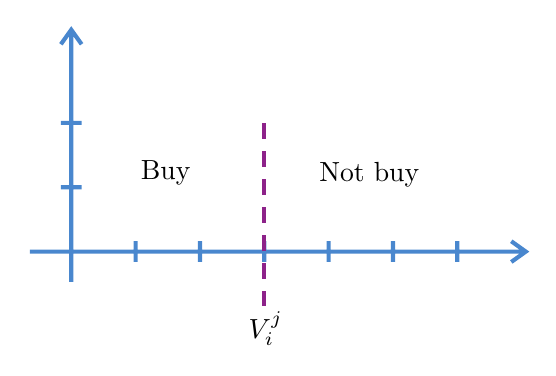
\begin{tikzpicture}[x=0.75pt,y=0.75pt,yscale=-1,xscale=1]
        %uncomment if require: \path (0,259); %set diagram left start at 0, and has height of 259

        %Shape: Axis 2D [id:dp048941842347560494] 
        \draw [color={rgb, 255:red, 73; green, 135; blue, 206 }  ,draw opacity=1 ][line width=1.5]  (41,184.39) -- (280,184.39)(61,77.5) -- (61,199) (273,179.39) -- (280,184.39) -- (273,189.39) (56,84.5) -- (61,77.5) -- (66,84.5) (92,179.39) -- (92,189.39)(123,179.39) -- (123,189.39)(154,179.39) -- (154,189.39)(185,179.39) -- (185,189.39)(216,179.39) -- (216,189.39)(247,179.39) -- (247,189.39)(56,153.39) -- (66,153.39)(56,122.39) -- (66,122.39) ;
        \draw   ;
        %Straight Lines [id:da5751643928734858] 
        \draw [color={rgb, 255:red, 141; green, 34; blue, 137 }  ,draw opacity=1 ][line width=1.5]  [dash pattern={on 5.63pt off 4.5pt}]  (154,122.5) -- (154,210.5) ;

        % Text Node
        \draw (145,212) node [anchor=north west][inner sep=0.75pt]   [align=left] {$\displaystyle V_{i}^{j}$};
        % Text Node
        \draw (93,139) node [anchor=north west][inner sep=0.75pt]   [align=left] {Buy};
        % Text Node
        \draw (179,140) node [anchor=north west][inner sep=0.75pt]   [align=left] {Not buy};


        \end{tikzpicture}\\
        The pedex i denotes the specific customer and j denotes the item if we have multiple items

    \subsubsection*{Demand Curve [Exam question]}
        The customer is modelled in terms of valuation over the good. The customer valuation is just the value that the customer gets when he or she acquires the good.
        Suppose to have multiple customers, potentially with different valuations. We can generate the demand curve.
        The demand expresses the number of customers that would buy a unit of the item at a given price. So, given all the potential customers and a price, we can count the
        number of customers whose valuation is larger than or equal to the given price. This number expresses the number of customers that would buy a unit of the item at the
        given price. Therefore this is the demand for the given price
        \vspace{5mm}



        \tikzset{every picture/.style={line width=0.75pt}} %set default line width to 0.75pt        

        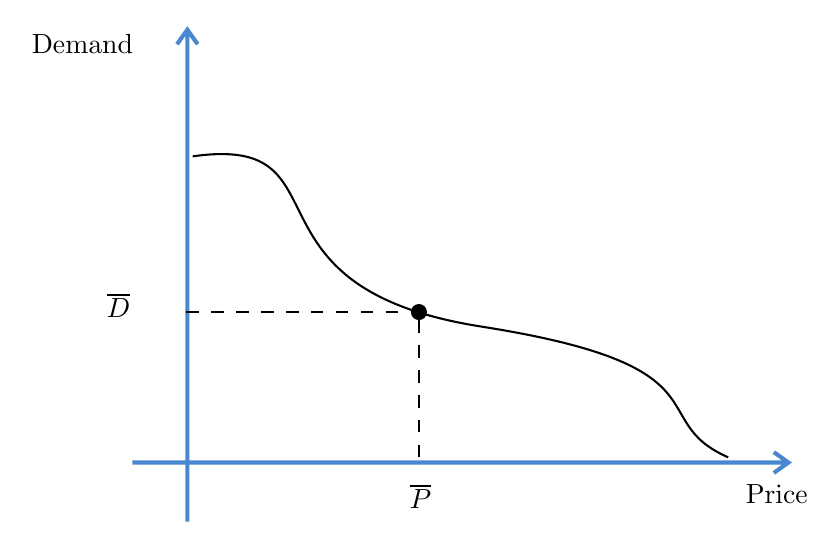
\begin{tikzpicture}[x=0.75pt,y=0.75pt,yscale=-1,xscale=1]
        %uncomment if require: \path (0,259); %set diagram left start at 0, and has height of 259
        %Shape: Axis 2D [id:dp12946740953043334] 
        \draw [color={rgb, 255:red, 73; green, 135; blue, 206 }  ,draw opacity=1 ][line width=1.5]  (62,217.01) -- (378,217.01)(88.44,8.5) -- (88.44,245.5) (371,212.01) -- (378,217.01) -- (371,222.01) (83.44,15.5) -- (88.44,8.5) -- (93.44,15.5)  ;
        %Curve Lines [id:da6847532330958823] 
        \draw    (91,69.5) .. controls (168,58.5) and (109,132.5) .. (230,151.5) .. controls (351,170.5) and (308,196.5) .. (349,214.5) ;
        %Straight Lines [id:da7194993832266894] 
        \draw  [dash pattern={on 4.5pt off 4.5pt}]  (88,144.5) -- (200,144.5) ;
        %Straight Lines [id:da8410910680110908] 
        \draw  [dash pattern={on 4.5pt off 4.5pt}]  (200,214.5) -- (200,144.5) ;
        \draw [shift={(200,144.5)}, rotate = 270] [color={rgb, 255:red, 0; green, 0; blue, 0 }  ][fill={rgb, 255:red, 0; green, 0; blue, 0 }  ][line width=0.75]      (0, 0) circle [x radius= 3.35, y radius= 3.35]   ;

        % Text Node
        \draw (194,226) node [anchor=north west][inner sep=0.75pt]   [align=left] {$\displaystyle \overline{P}$};
        % Text Node
        \draw (48,134) node [anchor=north west][inner sep=0.75pt]   [align=left] {$\displaystyle \overline{D}$};
        % Text Node
        \draw (356,226) node [anchor=north west][inner sep=0.75pt]   [align=left] {Price};
        % Text Node
        \draw (12,9) node [anchor=north west][inner sep=0.75pt]   [align=left] {Demand};
        \end{tikzpicture}
        \\
        In economic literature, the demand curve is supposed to be given and therefore that a seller knows it before choosing the prices. This is not true in general and, in realworld settings, it is unlikely that the demand curve is known beforehand.
        Consider a simple example of real-world electronic commerce scenario. In this case the demand curve is not usually expressed in terms of the number of units one would sell given a price, but it is expressed in terms of the probability one would sell a unit given a price. This probability to sell a unit of good is usually called conversion rate.



    \subsubsection*{Demand Elasticity [Exam question]}
        In economics, a very important index is the demand elasticity. To define the elasticity, suppose to consider a point (bar P, bar D) on the curve, as  in the previous graph. Then we consider the derivative on that point $\dfrac{d \bar{D}}{d \bar{P}}$, then the elasticity is defined as the product between the derivative of the demand w.r.t. the price and the ratio between the price and the demand. In other words, the  elasticity corresponds to a normalisation of the derivative of the demand w.r.t. the price. 

        \begin{equation}
            \dfrac{\bar{P}}{\bar{D}}\dfrac{dD}{dP}  \left(\bar{P}\right)
        \end{equation}

    \subsubsection*{Conversion Rate}
    Now, let's go back to the demand curve: in the ecommerce example we talked about Conversion rate. Suppose to consider a price. We do not know a priori the conversion rate. What we need is to estimate the expected value of a random variable expressing the probability distribution that the customers will buy a unit of good at the given price. So we take a few samples and then we compute the envelope of the expected values of these random variables. So, in these settings, we should use the term “average demand curve”.
    \vspace{5mm}

    \tikzset{every picture/.style={line width=0.75pt}} %set default line width to 0.75pt        

    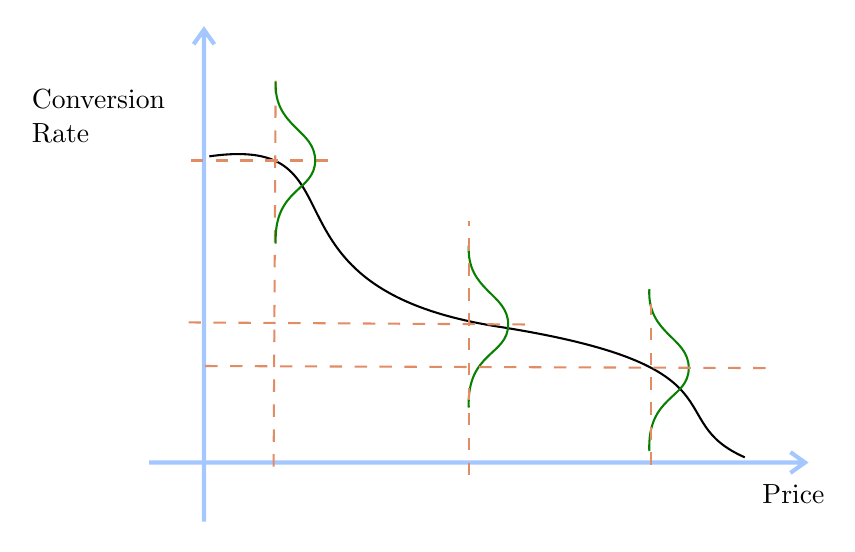
\begin{tikzpicture}[x=0.75pt,y=0.75pt,yscale=-1,xscale=1]
    %uncomment if require: \path (0,258); %set diagram left start at 0, and has height of 258

    %Shape: Axis 2D [id:dp4541058309510291] 
    \draw [color={rgb, 255:red, 164; green, 199; blue, 255 }  ,draw opacity=1 ][line width=1.5]  (62,217.01) -- (378,217.01)(88.44,8.5) -- (88.44,245.5) (371,212.01) -- (378,217.01) -- (371,222.01) (83.44,15.5) -- (88.44,8.5) -- (93.44,15.5)  ;
    %Curve Lines [id:da5616421774559066] 
    \draw    (91,69.5) .. controls (168,58.5) and (109,132.5) .. (230,151.5) .. controls (351,170.5) and (308,196.5) .. (349,214.5) ;
    %Straight Lines [id:da325441275083191] 
    \draw [color={rgb, 255:red, 226; green, 140; blue, 101 }  ,draw opacity=1 ] [dash pattern={on 4.5pt off 4.5pt}]  (122,219) -- (123,28) ;
    %Straight Lines [id:da050693299058129915] 
    \draw [color={rgb, 255:red, 226; green, 140; blue, 101 }  ,draw opacity=1 ] [dash pattern={on 4.5pt off 4.5pt}]  (148,71.5) -- (81,71.5) ;
    %Curve Lines [id:da17768048782056867] 
    \draw [color={rgb, 255:red, 7; green, 128; blue, 0 }  ,draw opacity=1 ]   (123,33.5) .. controls (122,55.5) and (142,56.5) .. (142,71.5) .. controls (142,86.5) and (122,84.5) .. (123,111.5) ;
    %Curve Lines [id:da7368317615637106] 
    \draw [color={rgb, 255:red, 7; green, 128; blue, 0 }  ,draw opacity=1 ]   (216,112.5) .. controls (215,134.5) and (235,135.5) .. (235,150.5) .. controls (235,165.5) and (215,163.5) .. (216,190.5) ;
    %Straight Lines [id:da7090676763726405] 
    \draw [color={rgb, 255:red, 226; green, 140; blue, 101 }  ,draw opacity=1 ] [dash pattern={on 4.5pt off 4.5pt}]  (243,150.5) -- (80,149.5) ;
    %Straight Lines [id:da9097372088280646] 
    \draw [color={rgb, 255:red, 226; green, 140; blue, 101 }  ,draw opacity=1 ] [dash pattern={on 4.5pt off 4.5pt}]  (216,223) -- (216,100.5) ;
    %Curve Lines [id:da3317304788672115] 
    \draw [color={rgb, 255:red, 7; green, 128; blue, 0 }  ,draw opacity=1 ]   (303,133.5) .. controls (302,155.5) and (322,156.5) .. (322,171.5) .. controls (322,186.5) and (302,184.5) .. (303,211.5) ;
    %Straight Lines [id:da33745109904476855] 
    \draw [color={rgb, 255:red, 226; green, 140; blue, 101 }  ,draw opacity=1 ] [dash pattern={on 4.5pt off 4.5pt}]  (359,171.5) -- (86,170.5) ;
    %Straight Lines [id:da9275074383935265] 
    \draw [color={rgb, 255:red, 226; green, 140; blue, 101 }  ,draw opacity=1 ] [dash pattern={on 4.5pt off 4.5pt}]  (304,218) -- (304,140.5) ;

    % Text Node
    \draw (356,226) node [anchor=north west][inner sep=0.75pt]   [align=left] {Price};
    % Text Node
    \draw (4,36) node [anchor=north west][inner sep=0.75pt]   [align=left] {Conversion\\Rate};


    \end{tikzpicture}



    \chapter{Pricing}
    Now we'll dive into details of pricing strategies. We start with a recap of the different possible scenarios:
    \begin{itemize}
        \item \textbf{Monopoly}: there is only one seller in the market
        \item \textbf{Oligopoly}: we have a small number of seller in the market. In this case, the sellers are competing each other and the solution can be
        found by using the idea of Nash equilibrium provided in the field of game theory.
        \item \textbf{Competitive market}:  there are many sellers and the effect of every single seller to the market is negligible. In this case, a solution can
        be found by using other tools provided in the field of game theory. In particular, using market equilibria such as the Arrow-Debreu equilibrium.
    \end{itemize}


    Let's focus on the first case and define some variables:
    
    \[
        \begin{array}{rl}
            p & \textnormal{price} \\
            q(p) & \textnormal{(aggregate) demand at price $p$} \\
            c(q(p)) & \textnormal{cost of every item when $q(p)$ items are sold} \\
            \\
            p\,q(p) & \textnormal{revenue at price $p$} \\
            p\,q(p)-c(q(p)) & \textnormal{profit at price $p$} \\
        \end{array}
    \]
    The seller is obviously a profit maximizer and therefore he or she tries to maximize the value of the profit.

    
    \begin{tcolorbox}


        In the economic literature, the researchers use an alternative formulation where the seller chooses the quantity of units to sell and the optimal prices used is derived from the demand curve. Notice that this is possible only when the demand curve is known.
        \[
            \begin{array}{rl}
                q & \textnormal{demand} \\
                p(q) & \textnormal{price of the inverse demand curve at $q$} \\
                c(q) & \textnormal{cost of every item when $q$ items are sold} \\
                \\
                p(q)\,q & \textnormal{revenue at demand $q$} \\
                p(q)\,q-c(q) & \textnormal{profit at demand $q$} \\
            \end{array}
        \]
        
    \end{tcolorbox}

    
    At this point we want to maximize the revenue: the necessary condition to have a maximum is that the first derivative of the profit with respect to the quantity is zero.

    \vspace*{5mm}
    \tikzset{every picture/.style={line width=0.75pt}} %set default line width to 0.75pt        

    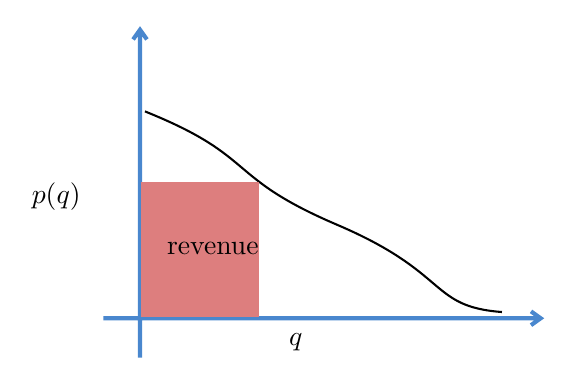
\begin{tikzpicture}[x=0.5pt,y=0.5pt,yscale=-1,xscale=1]
    %uncomment if require: \path (0,259); %set diagram left start at 0, and has height of 259
    
    %Shape: Axis 2D [id:dp22199722155980495] 
    \draw [color={rgb, 255:red, 73; green, 135; blue, 206 }  ,draw opacity=1 ][line width=1.5]  (62,217.01) -- (378,217.01)(88.44,8.5) -- (88.44,245.5) (371,212.01) -- (378,217.01) -- (371,222.01) (83.44,15.5) -- (88.44,8.5) -- (93.44,15.5)  ;
    %Curve Lines [id:da5208189169295399] 
    \draw    (92,67.5) .. controls (174,100.5) and (149,114.5) .. (231,149.5) .. controls (313,184.5) and (297,208.5) .. (350,212.5) ;
    %Shape: Rectangle [id:dp2894118965626169] 
    \draw  [draw opacity=0][fill={rgb, 255:red, 221; green, 126; blue, 126 }  ,fill opacity=1 ][dash pattern={on 0.84pt off 2.51pt}][line width=0.75]  (89.5,118.5) -- (174.31,118.5) -- (174.31,216.01) -- (89.5,216.01) -- cycle ;
    
    % Text Node
    \draw (194,226) node [anchor=north west][inner sep=0.75pt]   [align=left] {$\displaystyle q$};
    % Text Node
    \draw (8,117) node [anchor=north west][inner sep=0.75pt]   [align=left] {$\displaystyle p( q)$};
    % Text Node
    \draw (105.75,160) node [anchor=north west][inner sep=0.75pt]   [align=left] {revenue};
    
    
    \end{tikzpicture}

    \[
        \begin{array}{rl}
        \dfrac{d(p(q)\,q-c(q))}{dq} & = 0 \\
        \dfrac{dp(q)}{dq}\,q + p(q) - \dfrac{dc(q)}{dq} & = 0 \\
        \underbrace{\dfrac{dp(q)}{dq}\,q + p(q)}_{\textnormal{marginal revenue \textsf{MR$(q)$}}} & = \underbrace{\dfrac{dc(q)}{dq}}_{\textnormal{marginal cost \textsf{MC$(q)$}}} \\
        \end{array}
    \]\\
    Basically, the marginal revenue gives us the revenue provided by selling the last unit of good when the number of units sold is q. Similarly, the marginal cost gives us the cost due to selling the last unit of good when we number of units sold is q. Notice that both MR and MC are function in q.

    By solving the equation we can to take the value of q corresponding to the intersection of the curves MR and MC, then we can find the best price on the demand curve. 

    

    \tikzset{every picture/.style={line width=0.75pt}} %set default line width to 0.75pt        

    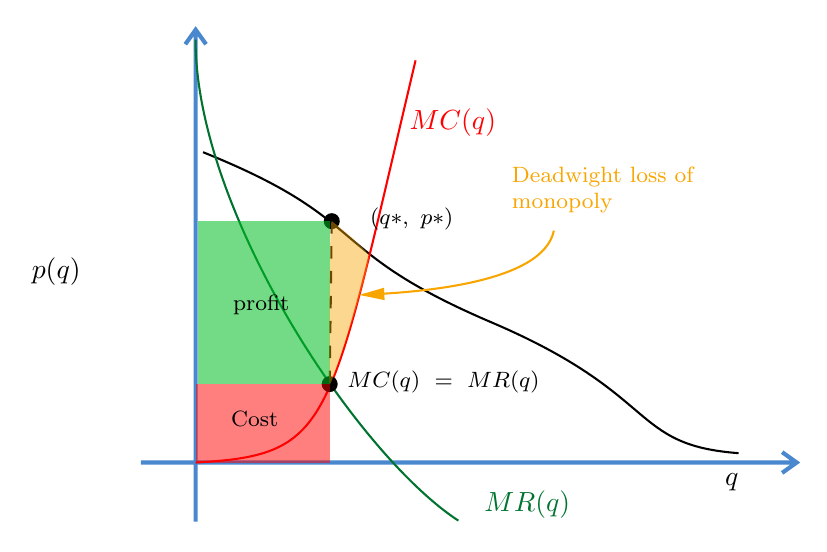
\begin{tikzpicture}[x=0.75pt,y=0.75pt,yscale=-1,xscale=1]
    %uncomment if require: \path (0,259); %set diagram left start at 0, and has height of 259

    %Shape: Axis 2D [id:dp3088745678143219] 
    \draw [color={rgb, 255:red, 73; green, 135; blue, 206 }  ,draw opacity=1 ][line width=1.5]  (62,217.01) -- (378,217.01)(88.44,8.5) -- (88.44,245.5) (371,212.01) -- (378,217.01) -- (371,222.01) (83.44,15.5) -- (88.44,8.5) -- (93.44,15.5)  ;
    %Curve Lines [id:da7637680178062856] 
    \draw    (92,67.5) .. controls (174,100.5) and (149,114.5) .. (231,149.5) .. controls (313,184.5) and (297,208.5) .. (350,212.5) ;
    %Curve Lines [id:da5593173840555432] 
    \draw [color={rgb, 255:red, 0; green, 115; blue, 47 }  ,draw opacity=1 ]   (88.38,13.25) .. controls (88.38,96.25) and (166.38,213.25) .. (215,245) ;
    %Curve Lines [id:da26640974665639683] 
    \draw [color={rgb, 255:red, 255; green, 0; blue, 0 }  ,draw opacity=1 ]   (88.44,217.01) .. controls (155.38,213.25) and (152.38,200.62) .. (194.38,23.25) ;
    %Straight Lines [id:da5751529990621342] 
    \draw  [dash pattern={on 4.5pt off 4.5pt}]  (154.01,100.72) -- (153.01,179.22) ;
    \draw [shift={(153.01,179.22)}, rotate = 90.73] [color={rgb, 255:red, 0; green, 0; blue, 0 }  ][fill={rgb, 255:red, 0; green, 0; blue, 0 }  ][line width=0.75]      (0, 0) circle [x radius= 3.35, y radius= 3.35]   ;
    \draw [shift={(154.01,100.72)}, rotate = 90.73] [color={rgb, 255:red, 0; green, 0; blue, 0 }  ][fill={rgb, 255:red, 0; green, 0; blue, 0 }  ][line width=0.75]      (0, 0) circle [x radius= 3.35, y radius= 3.35]   ;
    %Shape: Rectangle [id:dp4781715345765518] 
    \draw  [color={rgb, 255:red, 255; green, 0; blue, 0 }  ,draw opacity=0 ][fill={rgb, 255:red, 255; green, 0; blue, 0 }  ,fill opacity=0.5 ] (88.44,179.22) -- (153.01,179.22) -- (153.01,217.01) -- (88.44,217.01) -- cycle ;
    %Shape: Rectangle [id:dp3885539495326815] 
    \draw  [color={rgb, 255:red, 0; green, 0; blue, 0 }  ,draw opacity=0 ][fill={rgb, 255:red, 0; green, 190; blue, 34 }  ,fill opacity=0.55 ] (89.38,100.72) -- (153.01,100.72) -- (153.01,179.22) -- (89.38,179.22) -- cycle ;
    %Shape: Polygon Curved [id:ds8495726158605013] 
    \draw  [color={rgb, 255:red, 0; green, 0; blue, 0 }  ,draw opacity=0 ][fill={rgb, 255:red, 249; green, 165; blue, 0 }  ,fill opacity=0.44 ] (154.01,100.72) .. controls (155.34,101.6) and (169.68,113.27) .. (171.68,116.94) .. controls (173.68,120.6) and (153.34,181.94) .. (153.01,179.22) .. controls (152.68,176.5) and (152.68,99.84) .. (154.01,100.72) -- cycle ;
    %Curve Lines [id:da0038015277217622323] 
    \draw [color={rgb, 255:red, 249; green, 165; blue, 0 }  ,draw opacity=1 ]   (261.01,105.27) .. controls (255.81,130.95) and (194.52,135.07) .. (169.22,136.19) ;
    \draw [shift={(167.34,136.27)}, rotate = 357.61] [fill={rgb, 255:red, 249; green, 165; blue, 0 }  ,fill opacity=1 ][line width=0.08]  [draw opacity=0] (12,-3) -- (0,0) -- (12,3) -- cycle    ;

    % Text Node
    \draw (342,221) node [anchor=north west][inner sep=0.75pt]   [align=left] {$\displaystyle q$};
    % Text Node
    \draw (8,117) node [anchor=north west][inner sep=0.75pt]   [align=left] {$\displaystyle p( q)$};
    % Text Node
    \draw (226,229) node [anchor=north west][inner sep=0.75pt]  [color={rgb, 255:red, 0; green, 115; blue, 47 }  ,opacity=1 ] [align=left] {$\displaystyle MR( q)$};
    % Text Node
    \draw (190,45) node [anchor=north west][inner sep=0.75pt]  [color={rgb, 255:red, 255; green, 0; blue, 0 }  ,opacity=1 ] [align=left] {$\displaystyle MC( q)$};
    % Text Node
    \draw (171,93) node [anchor=north west][inner sep=0.75pt]  [font=\footnotesize] [align=left] {$\displaystyle (q*,\ p*)$};
    % Text Node
    \draw (160,171.5) node [anchor=north west][inner sep=0.75pt]  [font=\footnotesize] [align=left] {$\displaystyle {\textstyle MC( q) \ =\ MR( q)}$};
    % Text Node
    \draw (104,191) node [anchor=north west][inner sep=0.75pt]  [font=\footnotesize,color={rgb, 255:red, 0; green, 0; blue, 0 }  ,opacity=1 ] [align=left] {Cost};
    % Text Node
    \draw (105,135) node [anchor=north west][inner sep=0.75pt]  [font=\footnotesize] [align=left] {profit};
    % Text Node
    \draw (239.33,73.09) node [anchor=north west][inner sep=0.75pt]  [font=\footnotesize,color={rgb, 255:red, 249; green, 165; blue, 0 }  ,opacity=1 ] [align=left] {Deadwight loss of \\monopoly};


    \end{tikzpicture}


    We can see in the graph that the area given by the green and red boxes is the revenue, while the green box is the profit and the red area is the cost.
    Notice that the marginal cost at the optimal price is much lower than the price applied for that quantity of items sold. Consider instead the point at the intersection between the curve of the marginal cost and the demand curve. The seller could sell a number of units equal to the quantity corresponding to that point. This would allow for larger number of customers to get the good.But such a point is optimal from a social view. It is maximizing the number of units sold. However, this quantity and the corresponding best price is not optimal for the seller since the profit of the seller is zero.

    The area in orange corresponds to the inefficiency of the market due to the seller. In other words, the seller, being selfish, does not allow the market to be efficient. This area is called deadweight loss of monopoly.
